\documentclass{article}
\usepackage{graphicx} % Required for inserting images
\usepackage{amsmath}
\usepackage{wrapfig}
\usepackage{float}
\usepackage{biblatex} %Imports biblatex package
\addbibresource{sample.bib} %Import the bibliography file


\title{assignment1}
\author{ESSA.ALQALLAF    222121385}

\date{February 2024}

\begin{document}

\maketitle

\section{Graphs}
Graphs consist of two main elements which are vertices and edges, and they can be directed and undirected.  Usually, a graph is represented as (V, E) V denotes vertices and E denotes edges and both form a graph. Graphs have many applications they are used in many fields and it one of the most significant theory in computer science, so they are used in many applications like data structures and deep learning (GNN).  
Example:
\begin{figure}[H]

    \centering
    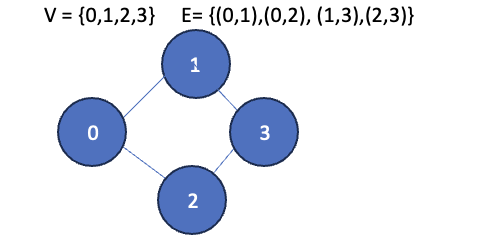
\includegraphics[width = \linewidth]{aa1.png}
    
\end{figure}

\section{Machine Learning}
Machine learning (ML) is a technique of making a computer think and solve problems by itself by training it through known data.  ML is a sector of Artificial intelligence, and it has four core types that will be discussed.
\subsection{Supervised}
Supervised learning is training the model on input and output and linking them with each other, so it takes (labeled dataset) which are output and inputs, and does two processes training and validation. For Example, by collecting labeled images of cars and planes and feeding them to a supervised learning algorithm, the machine will train a model that differentiates between them and will be able to detect cars and planes. Moreover, it has many applications that are used nowadays like fraud detection, email spam detection, and Recommendation systems.



\subsection{Unsupervised}
Unsupervised learning is a technique of using unlabeled data to determine patterns and relations. Therefore, it is used to find patterns in data that can be used for certain determinations like data exploration and visualization.  For example, soccer clubs could collect their players’ data from games and try to detect how they can improve by analyzing the weak aspects.

\subsection{Semi-supervised}
It is a mixture of supervised and unsupervised learning types, so it is a process of feeding labeled and unlabeled data to machine learning and through trained labeled data the algorithms can detect unlabeled objects. For example, feeding semi-supervised algorithms with labeled rulers and pens and unlabeled pencils. Then I train them the system will be able through the model to detect pencils. Furthermore, it has many applications like NLP and object recognition.

\subsection{Reinforcement}
Is a machine learning method that depends on reward, try, and error. So, in this technique, the system will train the data by rewarding the system each time it does something right to learn a certain behavior that is determined by the model. It has numerous applications such as robotics, finance, and game AI.
\section{Graph Neural Networks (GNN)}
GNN is a great technique for utilizing graphs to analyze and come up with new results, so it is used heavily in a lot of science fields to come up with solutions for some problems.  GNN algorithms focus on utilizing the neighbors by doing some math to get results that solve a desired problem. Therefore, the output can be a graph that has a lot of information in GNN algorithms and the outputs will be calculated by hidden layers that do some math utilizing the neighbors in a graph and then generate a result or a solution.  GNN has fruitful applications in real life like inventing medicines and automatous vehicles.

\cite{Distill1}
\cite{geeks1}
\cite{geeks2}
\cite{med}

\printbibliography
\end{document}
